



\subsection{Related Work}
\begin{figure}[t]
  \centering
  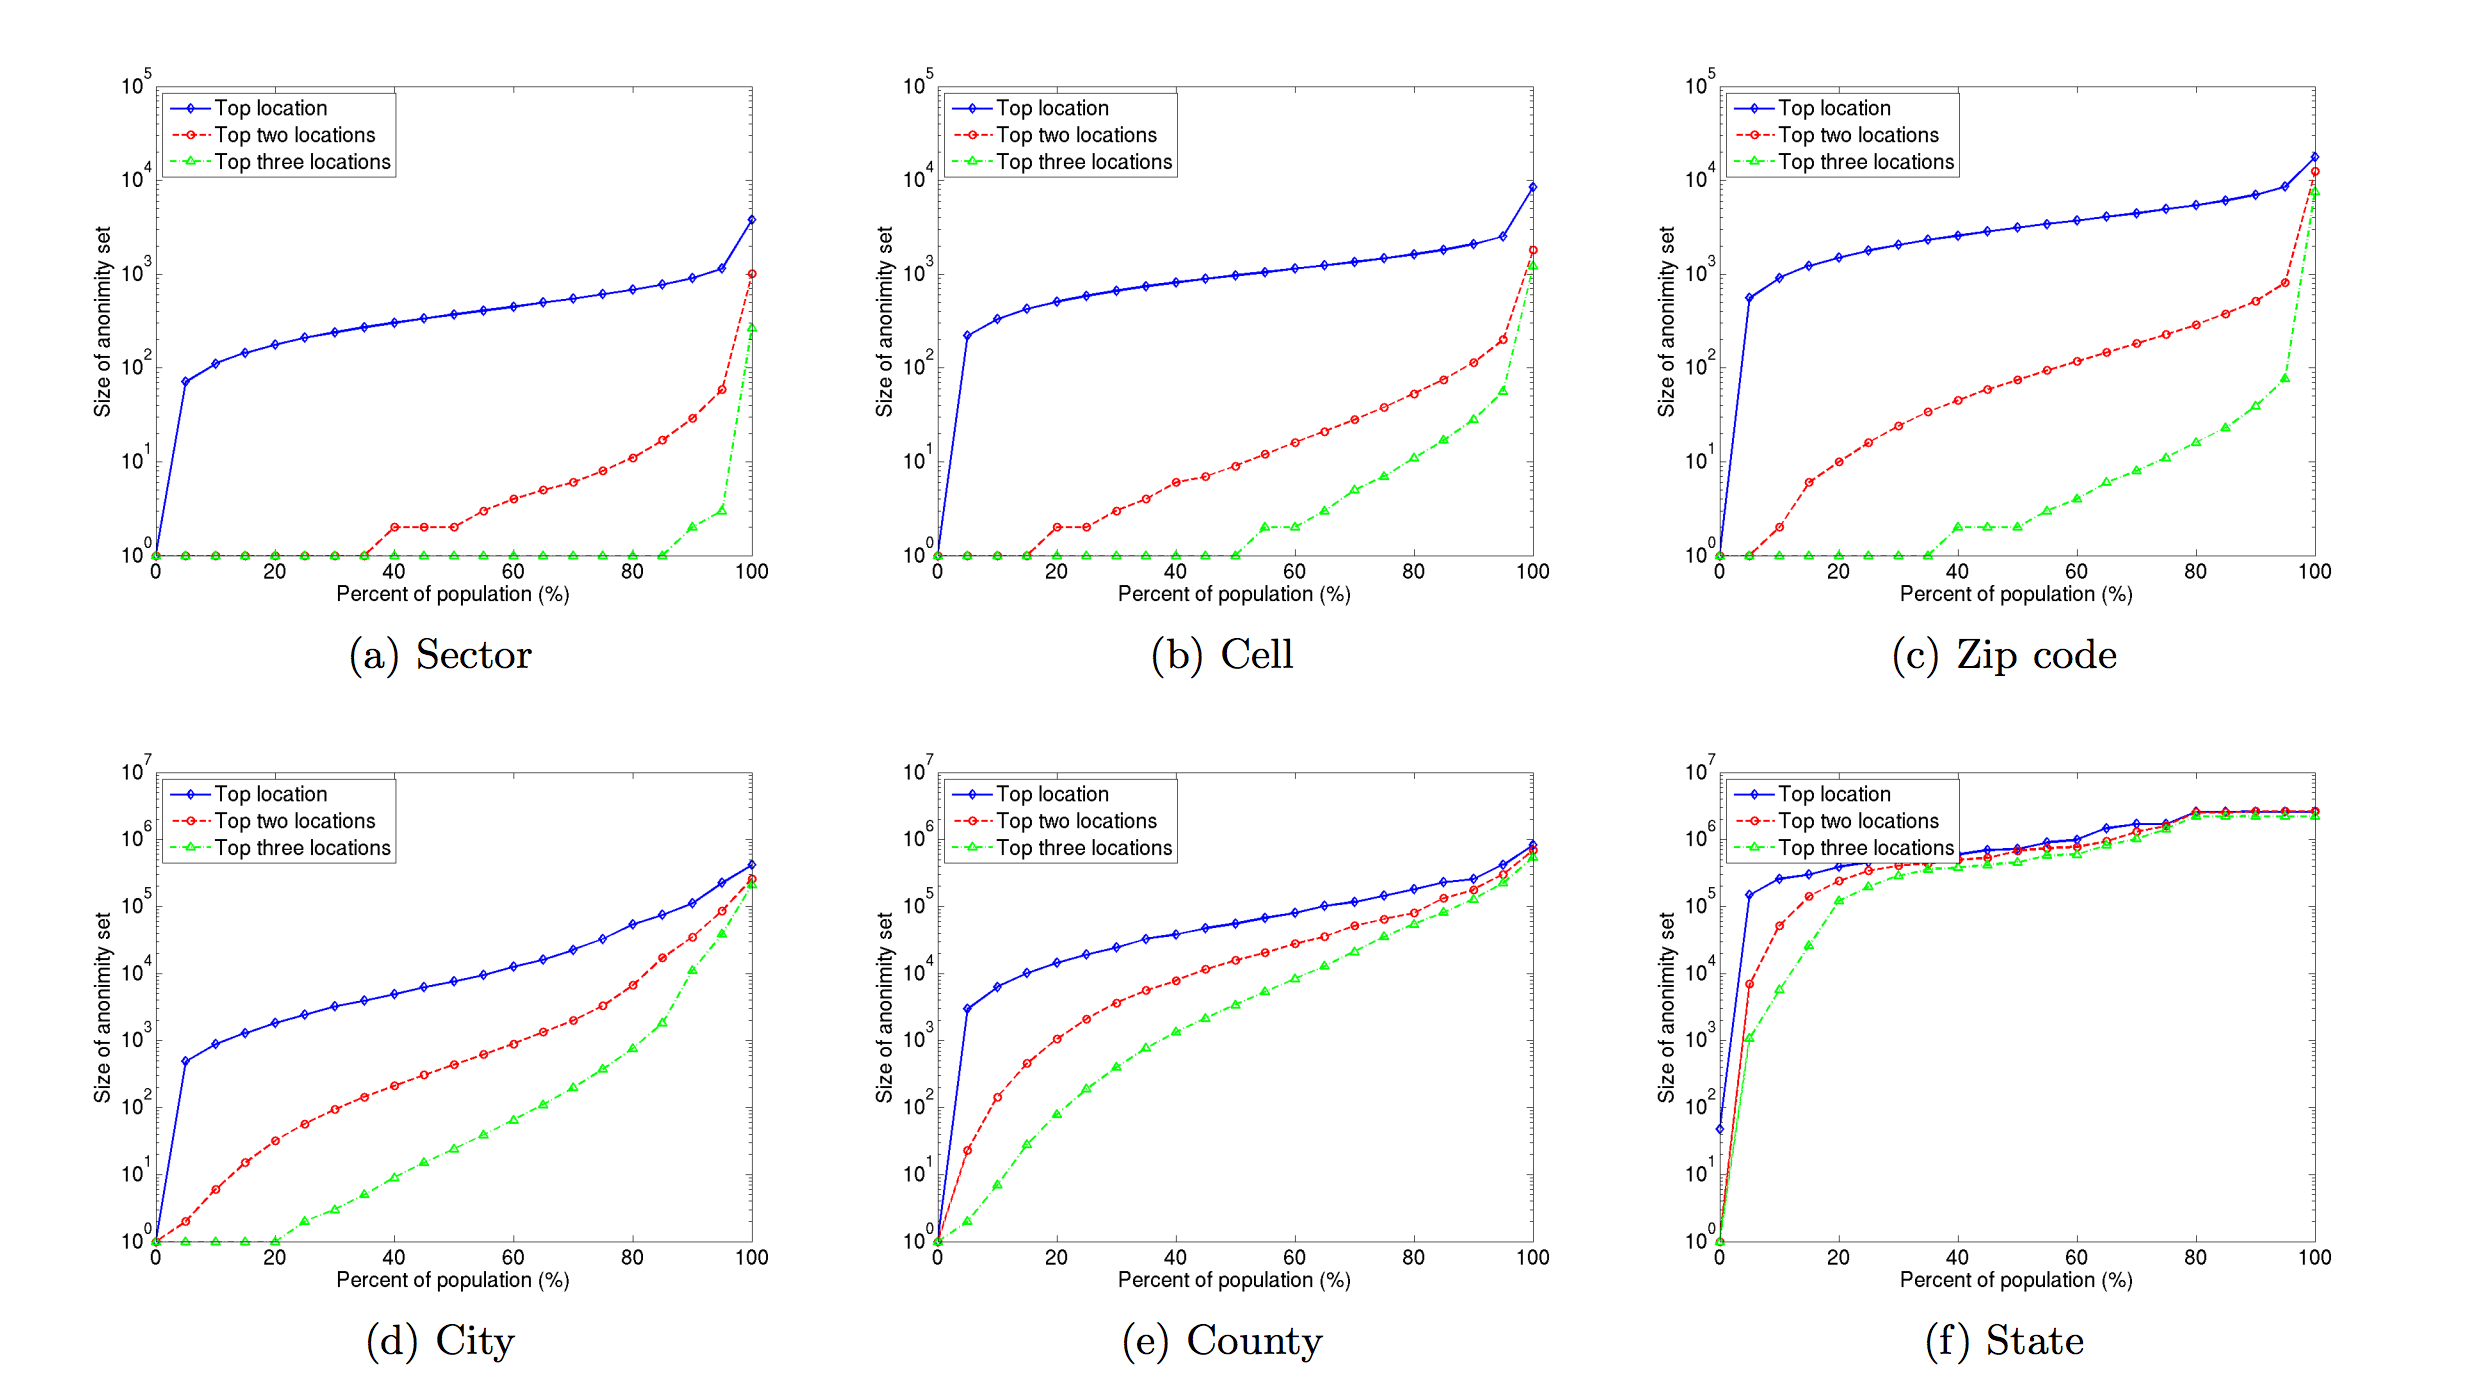
\includegraphics[width=\linewidth]{fig/zang_bolot.png}
  \caption{Figure from~\cite{Zang:2011hk} depicting the size of anonymity sets for top $n$ most visited location of users.
           Locations are varied in granularity, from cell sectors to US states.}
  \label{fig:zang_bolot}
\end{figure}

Location data for individuals is highly unique and thus difficult to anonymize.
The first large-scale study of the $k$-anonymity of location data was appropriately titled ``Anonymization of Location Data Does Not Work"~\cite{Zang:2011hk}.
The paper used data from cell phone call detail records (or CDR, see~\chap{sec:background}) for 25 million United States users over a 3 month period.
The authors represents each user as simply their top $n$ most visited locations, varying $n$ from 1 to 3.
Additionally, the authors varied the granularity of the locations, with the smallest as cell sector and the largest as state.
Remarkably, using 3 locations at a cell level made half of all users completely unique, and 3 locations a sector level made 85\% of all users unique.
A figure detailing this result and results for other granularities and values of $n$ is depicted in~\fig{fig:zang_bolot}.
The authors went on to analyze the impact of geography (comparing different states and cities), mobility (distances between top locations), and social networks on anonymity.


The Montjoye nature report


\subsection{Completed Work}
% Completed work introduction
I have investigated the anonymity of location data for users

\subsubsection{Linking Users Across Domains with Location Data}
% Background...
Although prior work showed location to be highly \emph{unique} and thus posibly \emph{vulnerable} to de-anonymization, no data was actually de-anonymized in practice.
Indeed, just because a data source is highly unique does not mean it can be de-anonymized.
For example, much of cryptography relies on creating highly unique but unpredictable sequences of numbers.
To put it more concretely, imagine that each individual had a die with 1000 sides, and each side represented a location.
If, quite hypothetically, humans decided where to go next by rolling this die, their movements would look very unique.
However, since the movements are random and unpredictable, my movements from different time periods will be indistinguishable from those of a different individual.

TODO: put some math here?

Another possibile break in the argument that uniqueness implies vulnerability is the important factor of sampling.
The datasets dealt with here (phone records, social media posts) are all \emph{actively} collected: each data point exists if and only if the user has taken an action.
Intuitively, the location data from different sampling data sources should look very different.
An individual may be more likely to make phone calls in quiet places, like the home or office, and take geotagged location photos in popular tourist destinations or restaurants.

TODO: put some math here?

In ``Linking Users Across Domains with Location Data", published at WWW in 2016~\cite{riederer2016linking}, we tackled this problem, linking users across two entirely different datasets.

% Describe problem setting
\begin{figure*}[t]
  \begin{center}
    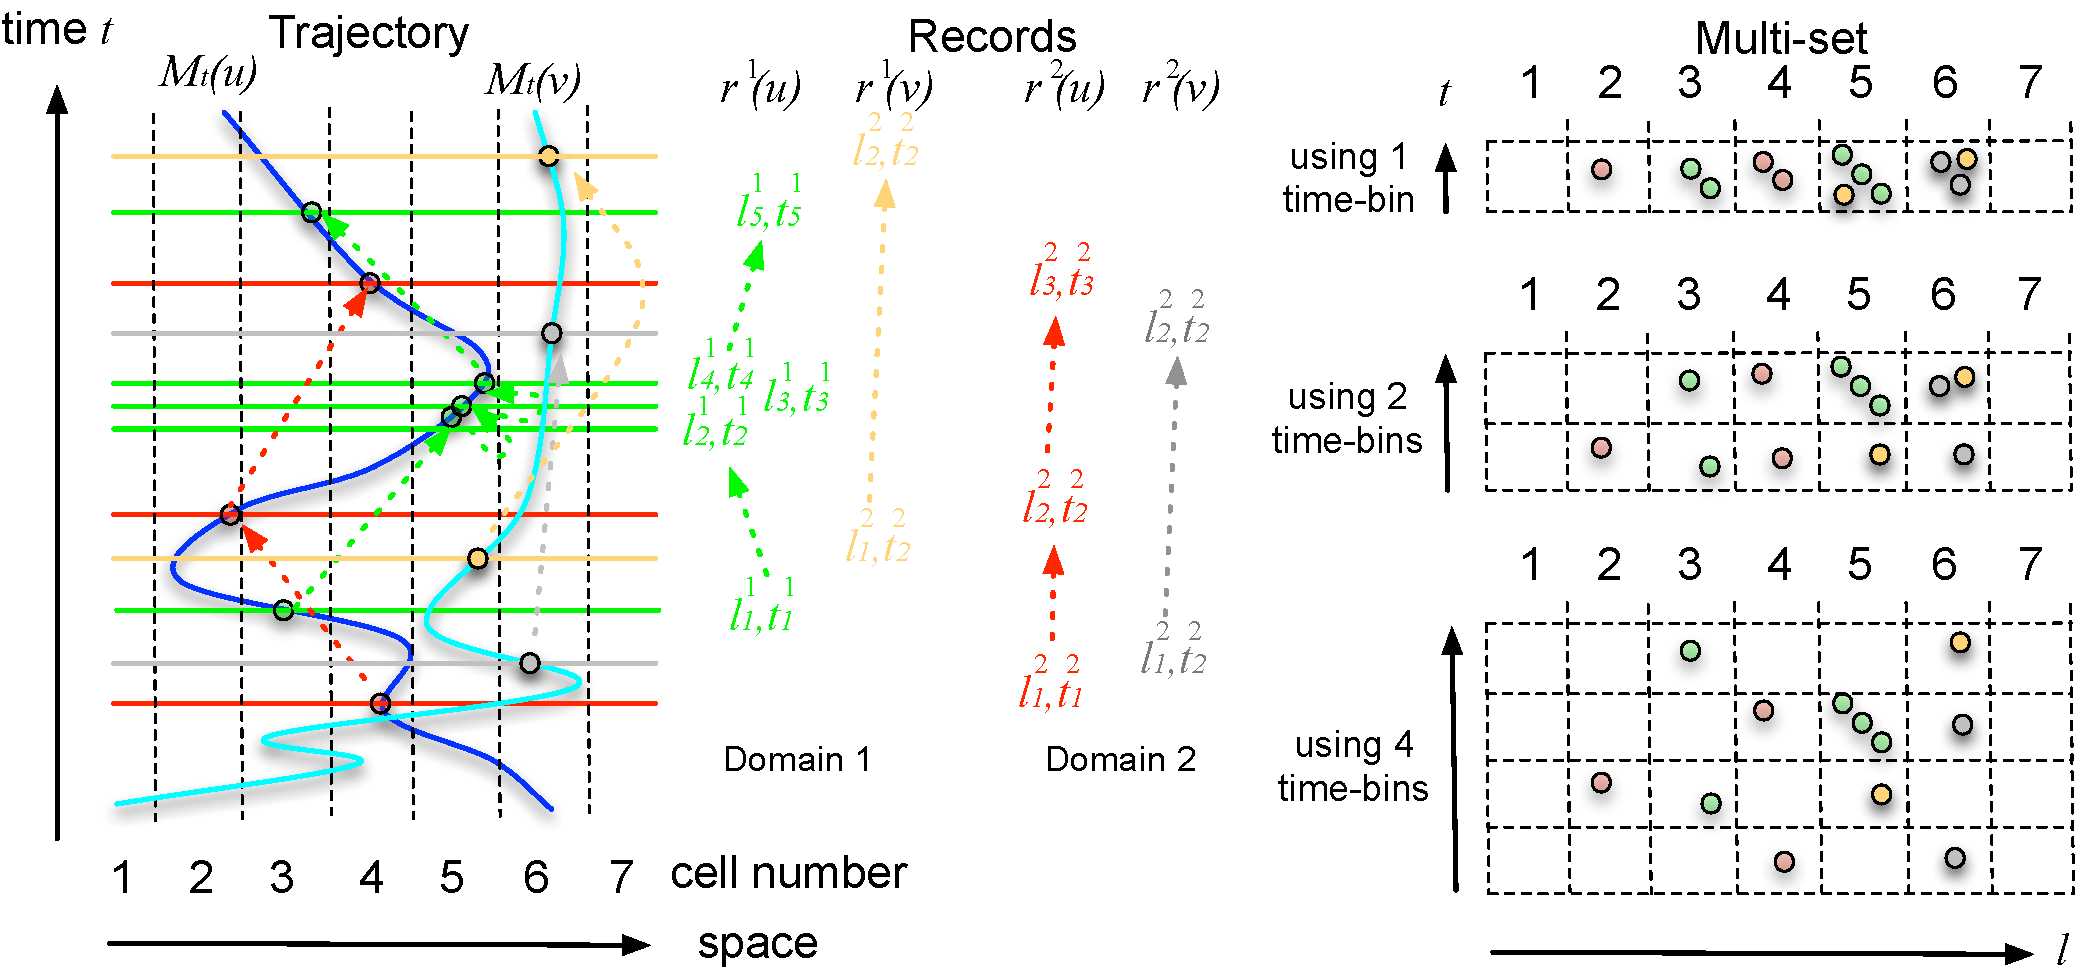
\includegraphics[width=0.65\linewidth]{fig/linking_explain.pdf}
  \end{center}
  \caption{Two space-time trajectories with associated footprints in two domains.}
  \label{fig:linking_explain}
\end{figure*}

% Describe problem
We formalized the problem in the following manner.
We defined $U$ and $V$ to be sets of $n$ user accounts in two separate domains.
Each account is a itself a set of spatiotemporal points $p$, where
\[ p = \langle u, l, t \rangle \]
with $u$ being a user ID unique to either $U$ or $V$, $l$ is a location, and $t$ is a time.
We denoted $\sigma_I$ to be a true (``identity'') mapping that correctly links the two accounts of the each user across $U$ and $V$.
The goal then, of this work, is to recover $\sigma_I$.
    
We made a series of simple assumptions about human mobility.
We broke time into discrete ``bins" of a certain length, and then declared the number of checkins a user has at each location in time bin to be Poisson distributed according to a rate paramater $\lambda$ unique to that time and place.
This is a simple but reasonable assumption, and Poisson distributions are often used to model rare events (like checkins).

This model generates the \emph{real world} mobility of a user.
We assume that this real world mobility is sampled independentally and randomly for the two different data sets with probability $p_U$ and $p_V$.

\fig{fig:linking_explain} provides a visual illustration.
On the left side of the image are two real world trajectories, denoted with a blue and turquoise line.
The x axis shows space and the y axis shows time.
The colored circles (red, green, gray and yellow) show times and places where the real world trajectories are sampled, with (for example) a geolocated photograph, phone call, or checkin.
The challenge is that we only see the green, yellow, red, and gray trajectories in the middle of the image, and we must figure out the true association across datasets.
In this example, red should go with green and gray with yellow.
On the right side of the image, the concept of time bins are illustrated.
We discretize time with varying sized time bins.
The top uses one large time bin, essentially ignoring time, whereas the bottom breaks time into four sections, essentially saying two locations are only the same if the checkins occur near one another in time.

% Describe algorithm
% Based on these assumptions, we were able to develop a maximum likelihood 

% Describe dataset
\begin{table*}
  \centering
  \begin{tabular}{llrrrrr}
    % \toprule
            &        & Number & Number  &   Median  &  Number   &           \\
    Dataset & Domain & Users & Checkins &  Checkins & Locations & Date Range\\
    \midrule
    FSQ-TWT   & Foursquare  & 862 & 13,177  & 8    & 11,265 & 2006-10 -- 2012-11 \\
              & Twitter     & 862 & 174,618 & 60.5 & 75,005 & 2008-10 -- 2012-11 \\
    \addlinespace
    IG-TWT    & Instagram   & 1717 & 337,934 & 93 & 177,430 & 2010-10 -- 2013-09 \\
              & Twitter     & 1717 & 447,366 & 89 & 182,409 & 2010-09 -- 2015-04 \\
    \addlinespace
    Call-Bank & Phone Calls       & 452 & $\sim$200k & $\sim$550 & $\sim$3500 & 2013-04 -- 2013-07 \\
              & Card Transactions & 452 & $\sim$40k & $\sim$60 & $\sim$3500 & 2013-04 -- 2013-07 \\
    % \bottomrule
  \end{tabular}
  \caption{Overview of datasets used in study. For FSQ-TWT and IG-TWT, number of locations refers to locations at a 4 decimal GPS granularity (position within roughly 10m).}
  \label{tab:link-data}
\end{table*}

We evaluated this algorithm on multiple real-world datasets.
Gathering the data in itself was a significant challenge, as each dataset needed to contain individuals with identities linked across two different data sources.
Collecting information from one data source is enough of a challenge by itself, given unexpected and changing data formats, connectivity problems, rate limits, and more.
Getting ground truth data across two datasets is thus more difficult, as two APIs need to be dealt with and user identities must be verified across the two.

We gathered three datasets:
\begin{itemize}
  % Data from foursquare checkins and geolocated tweets, from another paper.
  \item \textbf{Foursquare-Twitter} (FSQ-TWT): 
  checkin data from the location-based social networking and review site Foursquare \footnote{\url{https://foursquare.com/}} and geotagged updates from the microblogging site Twitter \footnote{\url{twitter.com}}. 
  This data was obtained in a prior work by other authors who allowed us to use their data~\cite{Zhang:2014ij}.
  We expect the behavior to be somewhat different across the two networks; Foursquare is primarily used to review restaurants, and Twitter is generally used.

  % Geolocated photos and geolocated tweets. Not the exact same. Got twitter account from profile. Medium difficulty.
  \item \textbf{Instagram-Twitter} (IG-TWT):
  Geolocated photographs from the image sharing site Instagram \footnote{\url{instagram.com}} and geotagged updates from the microblogging site Twitter.
  We first crawled Instagram, and then found users who had posted their Twitter usernames in their profiles.
  For each of these users, we used Twitter's API to crawl their public tweets.
  We expected this dataset to be the easiest to link, as there were high numbers of checkins on both sites for most users.

  % Cell phone calls (located to cell tower) and geocoded businesses.
  \item \textbf{Cell phone-Credit Card} (Call-Bank):
  Phone calls associated with geolocated cell towers (CDR) and credit or debit card transaction data associated with geocoded businesses, all from one G20 country.
  Locations were declared the same if the lat-lon of business was within a cell created via a Voronoi tesselation.
  This data was very sparse and the behaviors generating data seems to be very different in the two sets, making us hypothesize that we would have our worst results on it.
\end{itemize}

Statistics about these datasets is summarized in Table~\ref{tab:link-data}.

% Describe results
\begin{figure*}[th!]
  \centering
  \hspace{-0.7cm}
  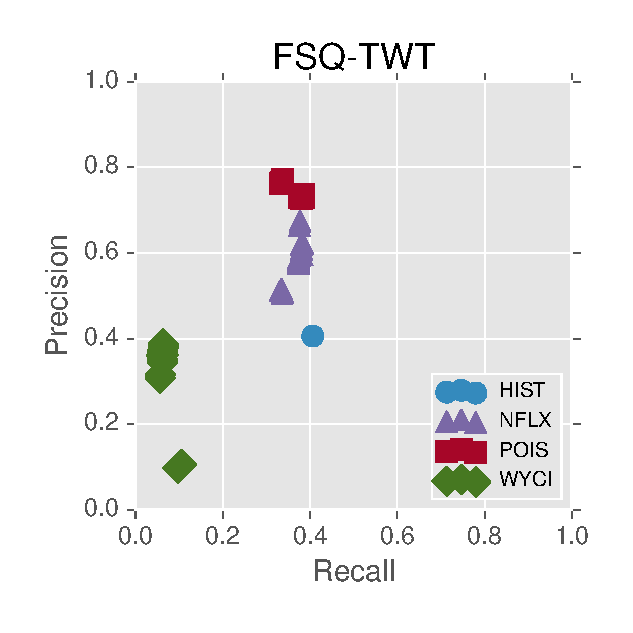
\includegraphics[width=0.35\linewidth]{fig/fs_scatter.eps}
  \hspace{-0.7cm}
  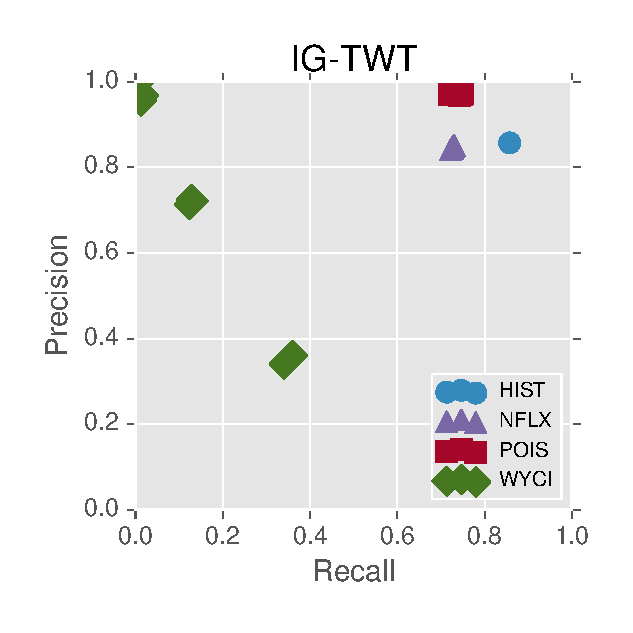
\includegraphics[width=0.35\linewidth]{fig/ig_scatter.eps}
  \hspace{-0.7cm}
  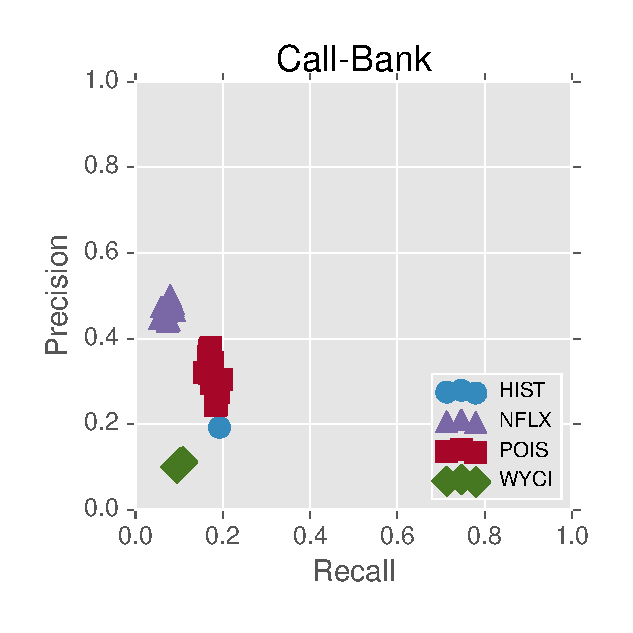
\includegraphics[width=0.35\linewidth]{fig/gd_scatter.eps}
  \caption{Precision and Recall plots for each dataset.}
  \vspace{1ex}
  \label{fig:link-prec-recall}
\end{figure*}

We now turn our attention to experimental performances of our algorithm. 
In Figure~\ref{fig:link-prec-recall}, we show the precision recall plots for our algorithm (for different eccentricity values) and for the other three reconciliation techniques: HIST, NFLX and WYCI. 
For our algorithm, we used estimated parameters and  for the other techniques, we used optimal parameters (found via exhaustive search).

There are several interesting observations that we can make on Figure~\ref{fig:link-prec-recall}. 
First, on the public dataset FQ-TWT our algorithm outperforms all prior methods (especially in precision). 
Nevertheless it is interesting to note that the precision of all methods is not ideal, probably due to sparsity of the data.

A second interesting observation is that our algorithm achieves very high precision when the dataset is more rich. 
In fact when we then turn our attention to our second dataset, the live service (IG-TWT) that we crawled, we obtain almost perfect precision. 
Note that not all the other techniques, for example NFLX, are able to leverage the denser data, as much.

Finally we test our method on a much more heterogeneous dataset (Call-Bank) that is also more realistic and sensitive. 
In this setting our algorithm outperforms previous techniques, with none of the previous algorithms able to achieve good precision and recall at the same time. 

% TODO(can possible add more results)
Other results found that our algorithms rapidly improved with more data.
Additionally, varying the size of timebins or the eccentricity parameter or number of terms did not have a large impact on results, meaning our algorithm's performance should remain stable to different sets of parameters.

% Conclusion?


\subsubsection{FindYou: A Personal Location Privacy Auditing Tool}

% TODO(cjr): Transition

FindYou has two main goals:
The first goal of our project is to inform users, regardless of technical skill, about what their location information can reveal. 
The second goal is to improve research on demographics and mobility by gathering a new dataset with the informed consent of interested users.

\begin{figure}[h]
  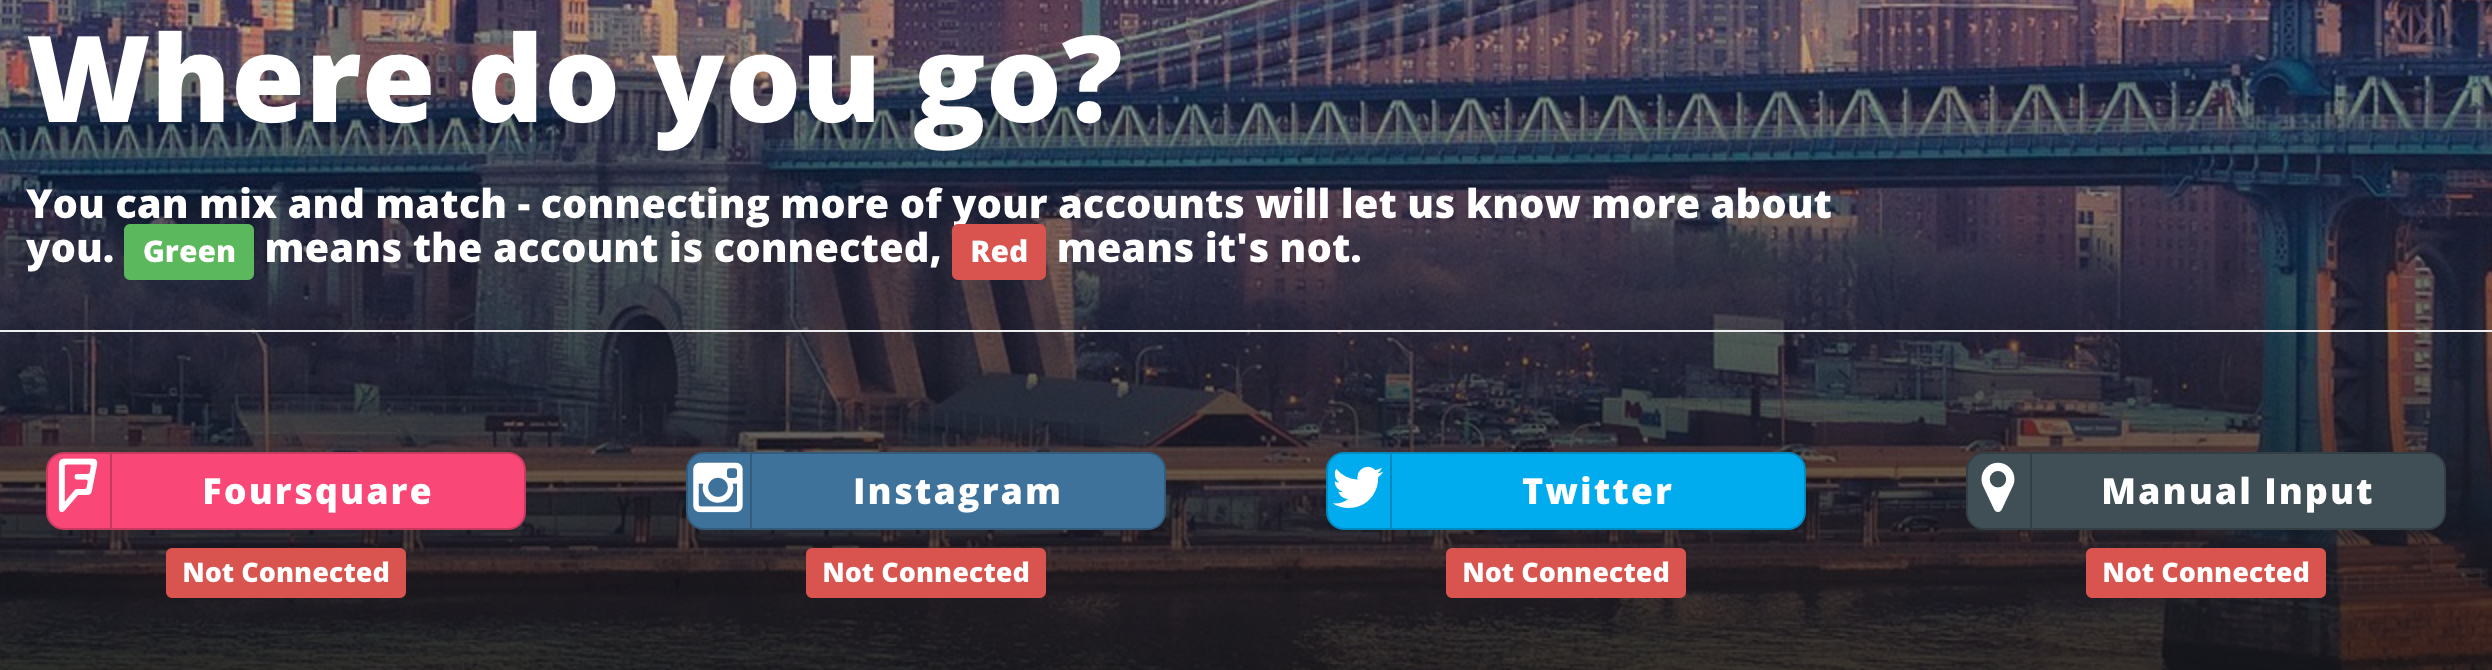
\includegraphics[width=\figwidth]{fig/findyou/connection.png}
  \caption{The user is presented with four different ways of connecting his or her location data to the app.}
  \label{fig:connection}
\end{figure}

\begin{figure}[h]
  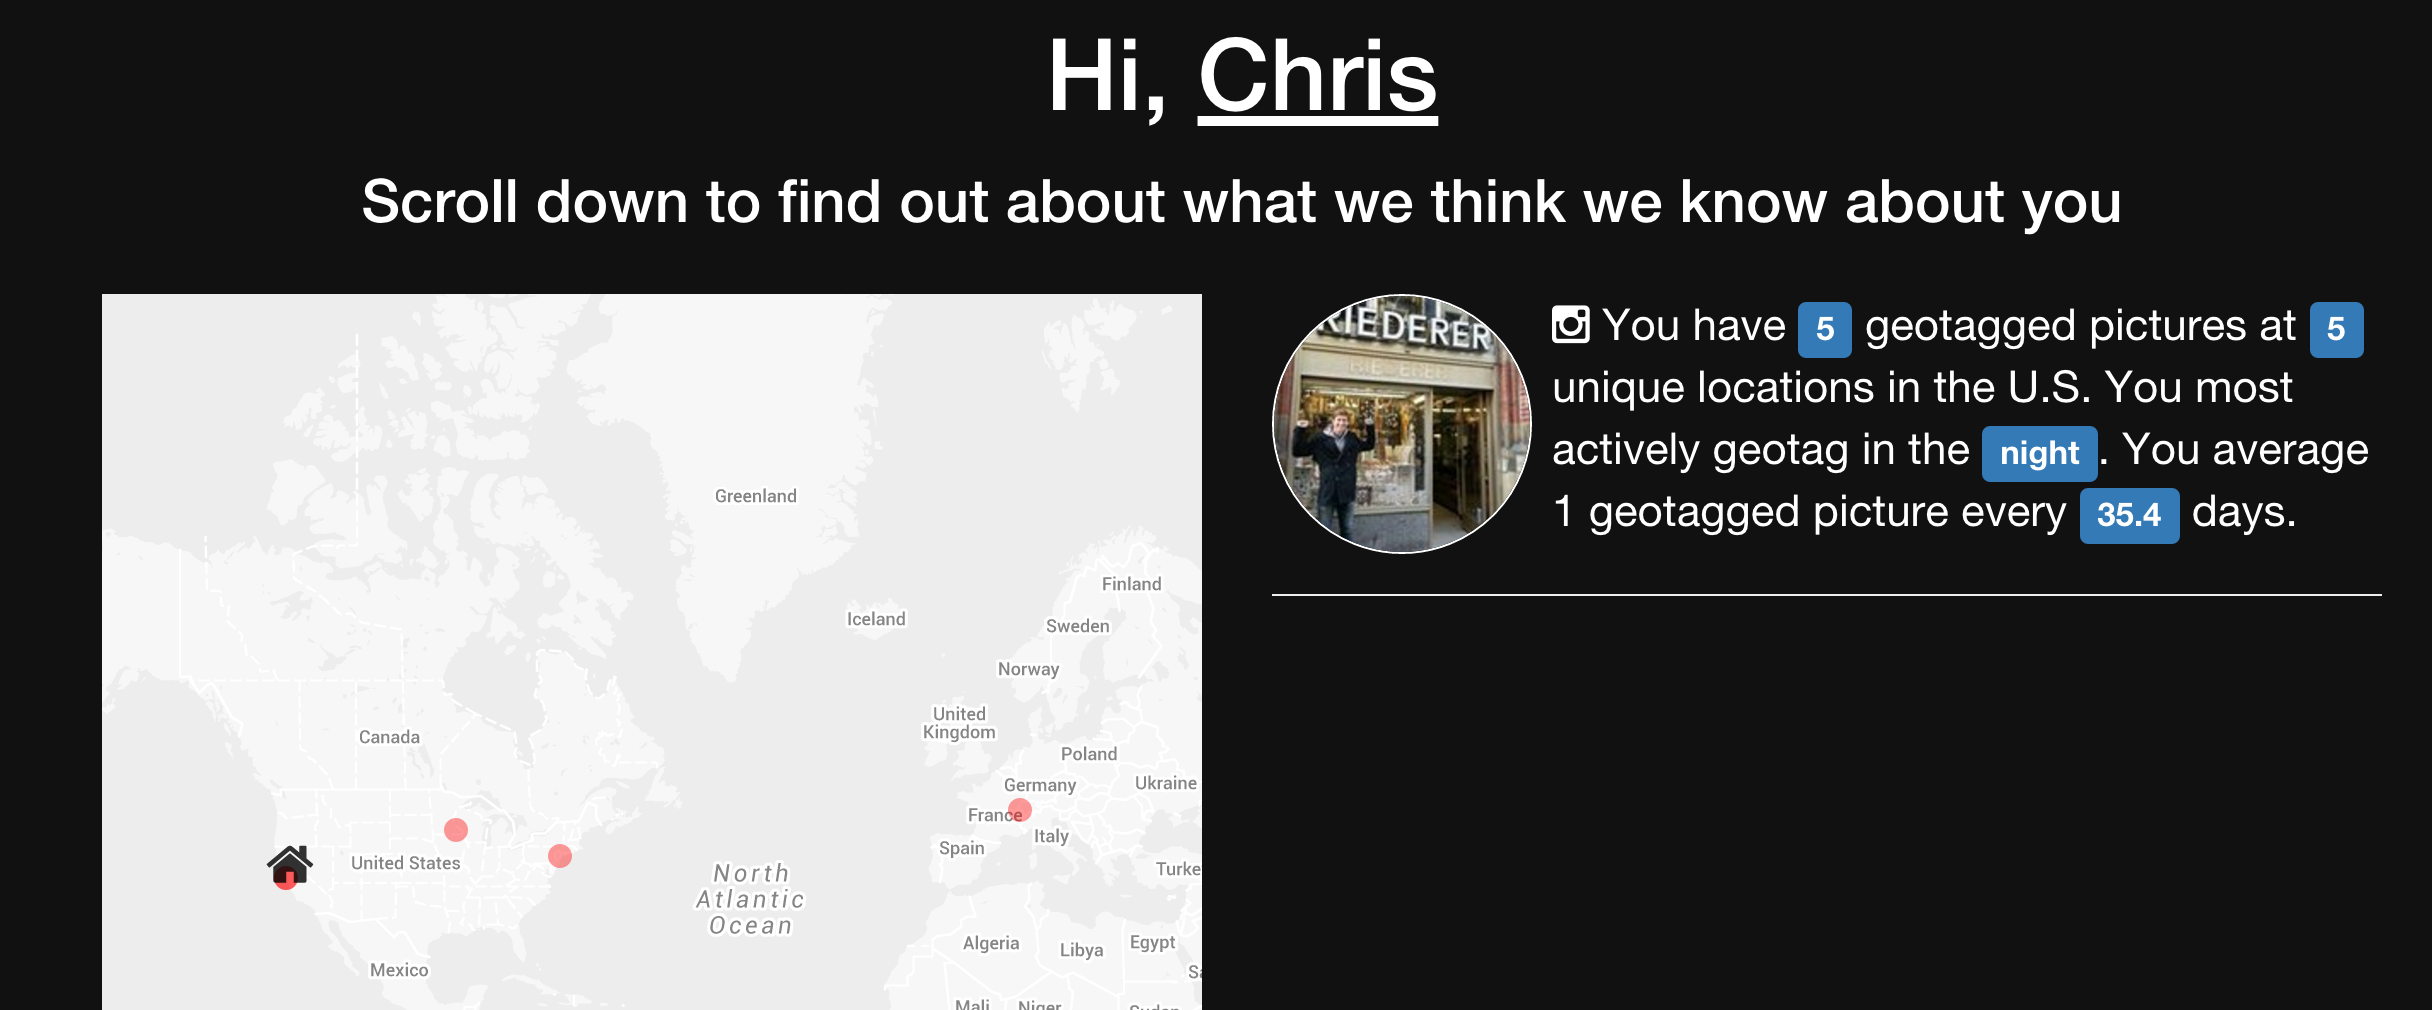
\includegraphics[width=\figwidth]{fig/findyou/overview.png}
  \caption{After connecting their data, the user sees an overview of their locations and imported data.}
  \label{fig:overview}
\end{figure}

\begin{figure}[h]
  
\includegraphics[width=\figwidth]{fig/findyou/home.png}
  \caption{We show a specific guess for the user's home location.}
  \label{fig:home}
\end{figure}

\begin{figure}[h]
  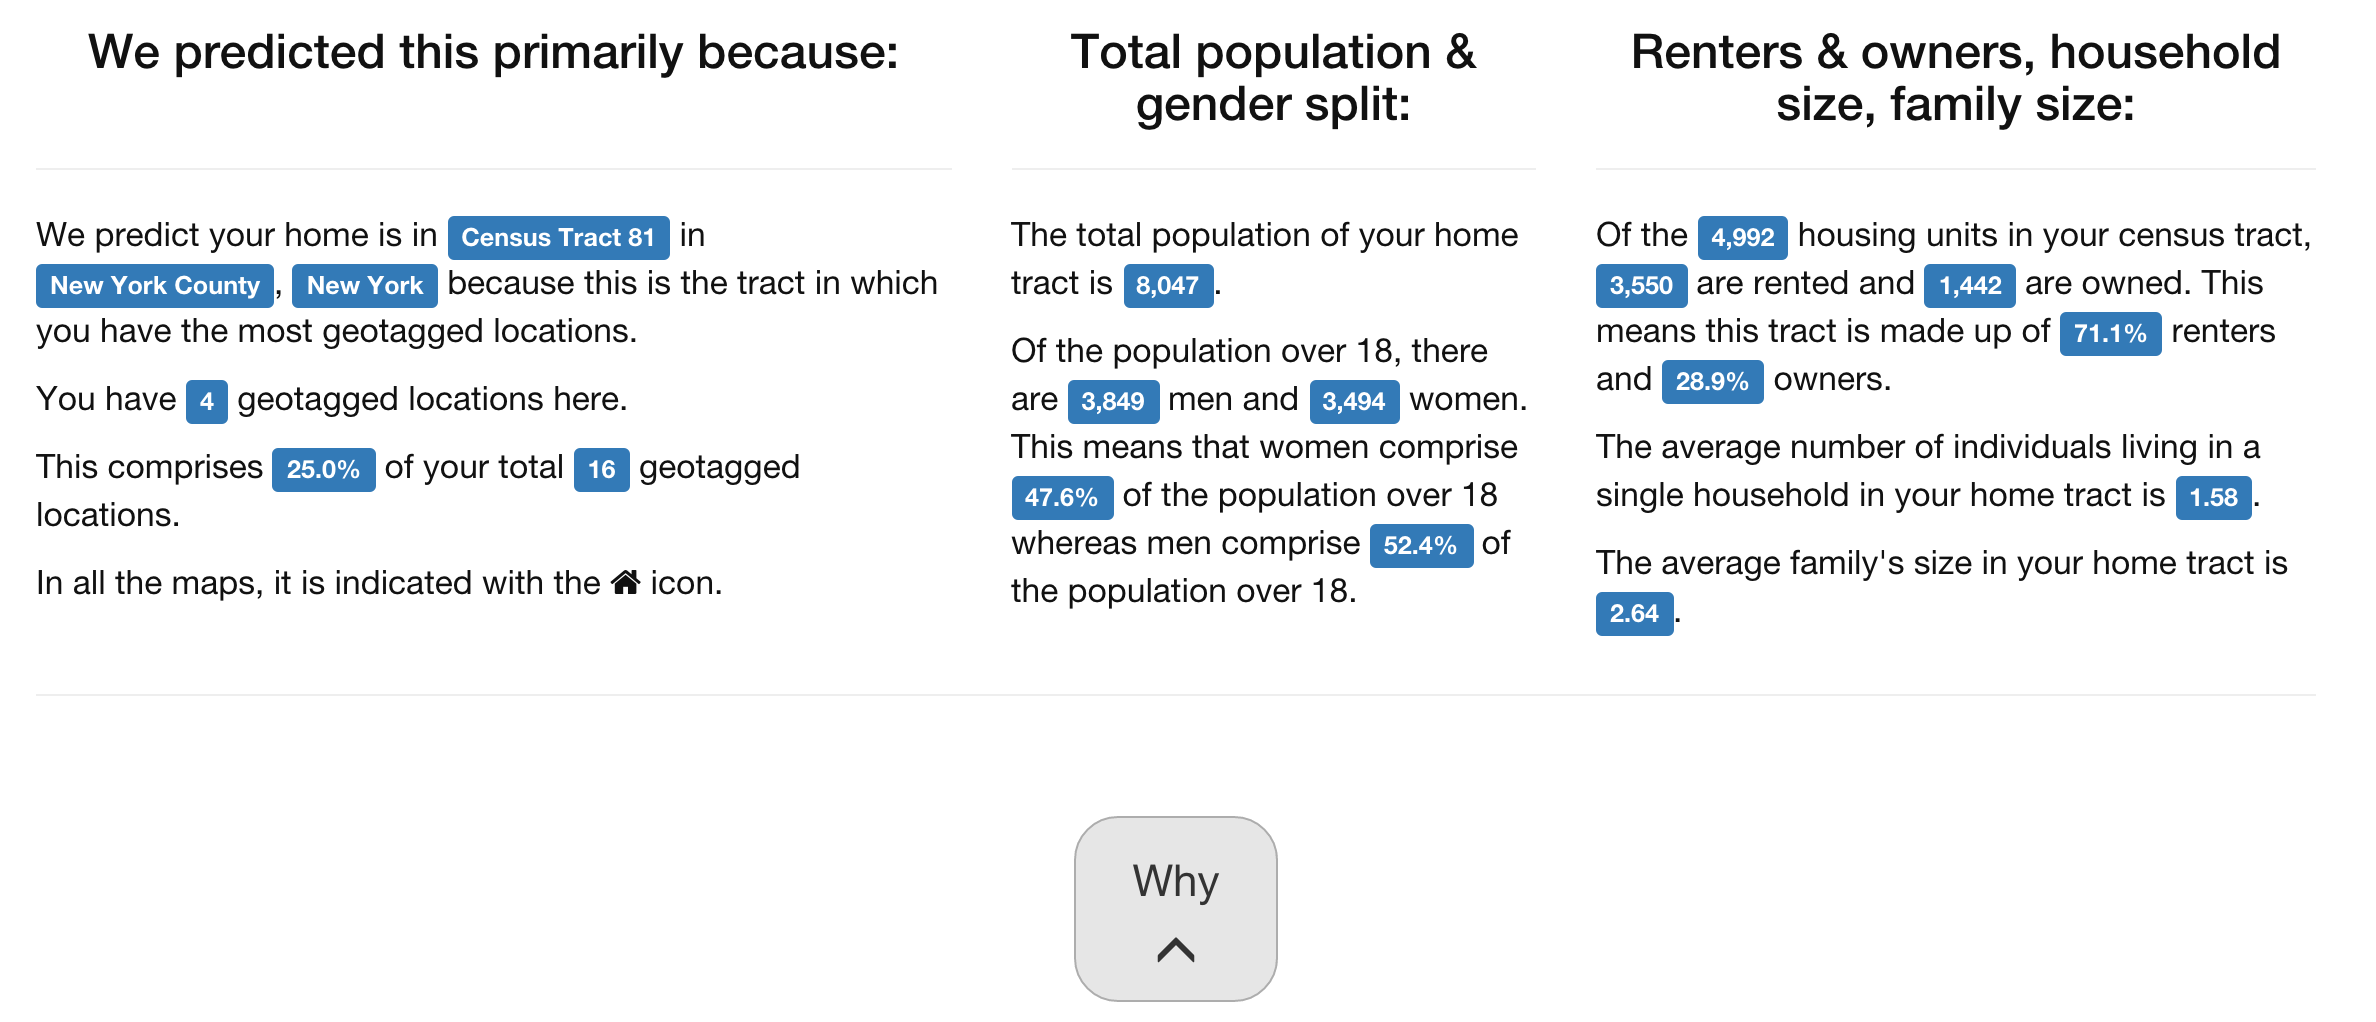
\includegraphics[width=\figwidth]{fig/findyou/home-detail.png}
  \caption{For all predictions, we show additional details about how we made this guess.}
  \label{fig:home-detail}
\end{figure}

\begin{figure}[h]
  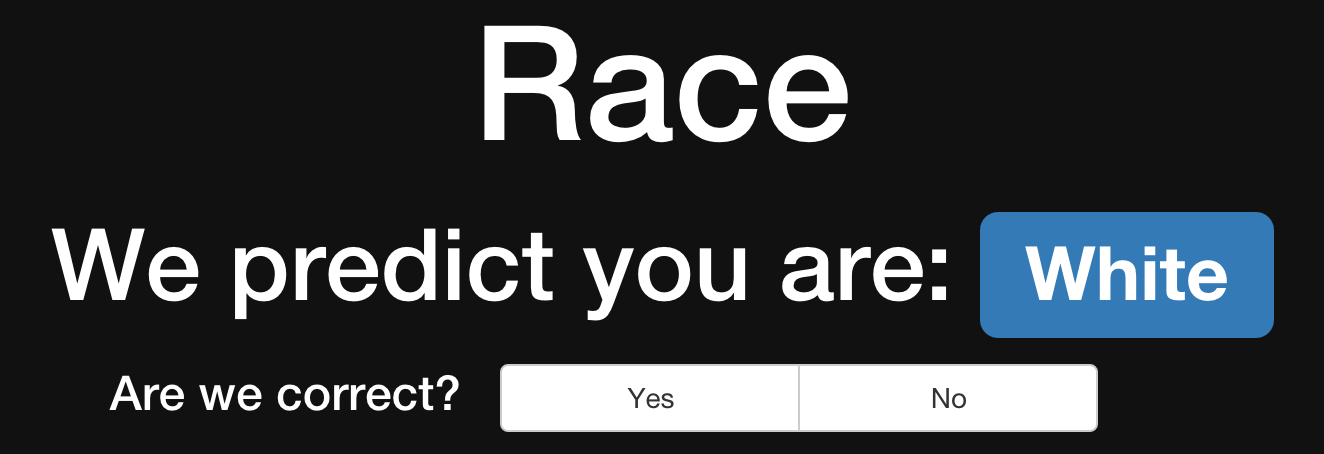
\includegraphics[width=\figwidth]{fig/findyou/race.png}
  \caption{The site predicts several demographic attributes, one of which is race. The user has the option to tell us if we are correct.}
  \label{fig:race}
\end{figure}

\begin{figure}
  \centering
  \begin{subfigure}[b]{.2\textwidth}
    \centering
    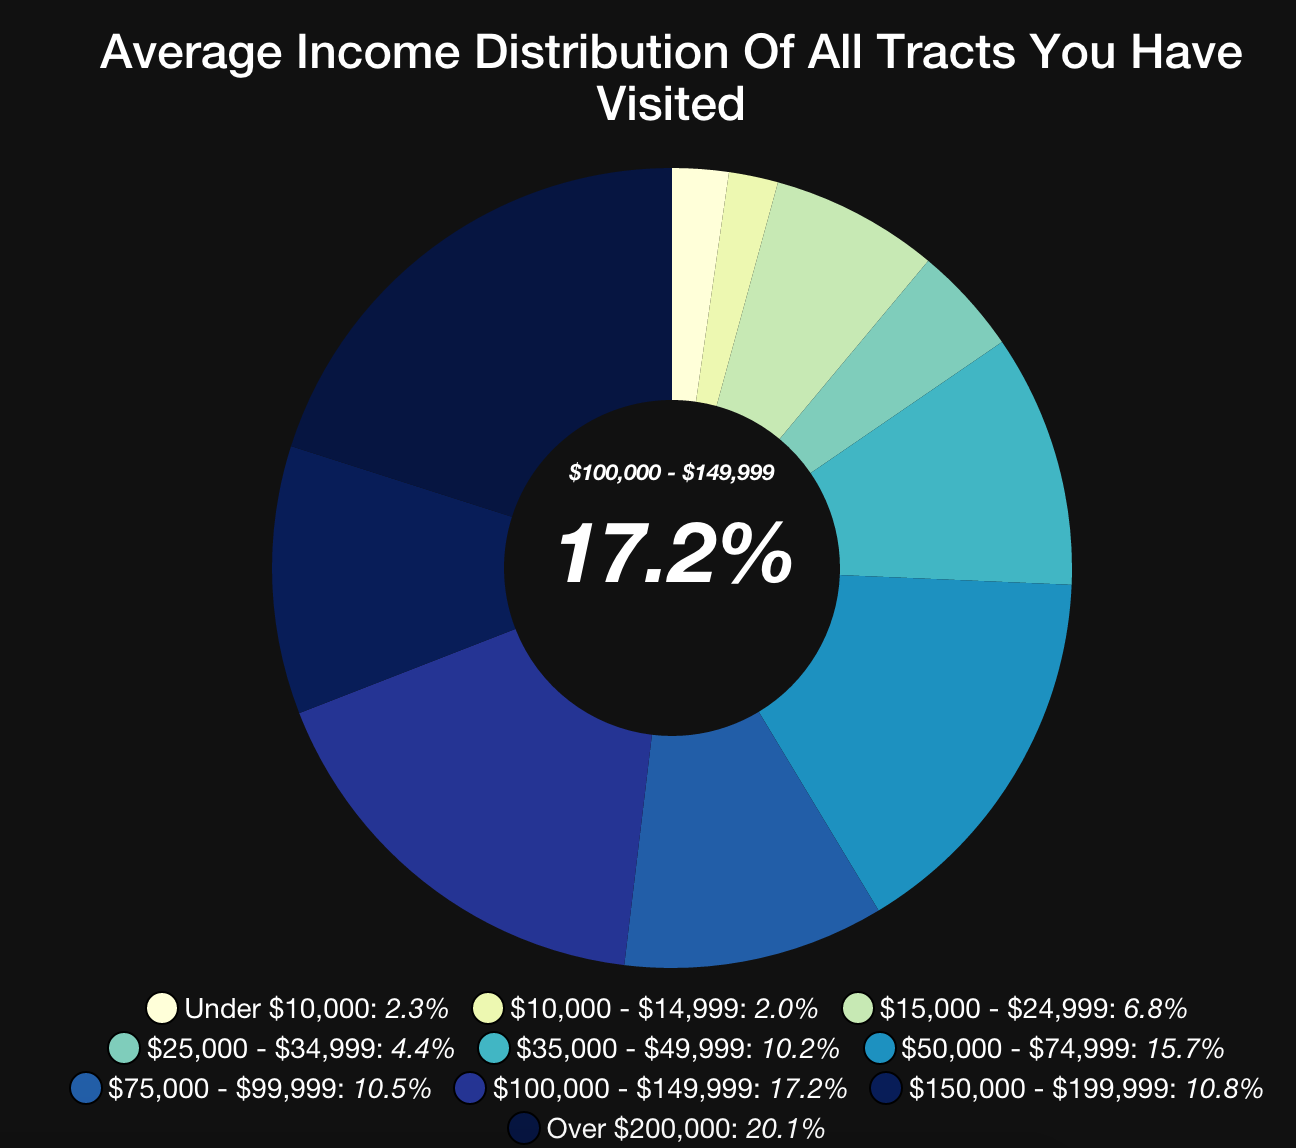
\includegraphics[width=\linewidth]{fig/findyou/donut.png}
    \caption{}
  \end{subfigure}
  \begin{subfigure}[b]{.2\textwidth}
    \centering
    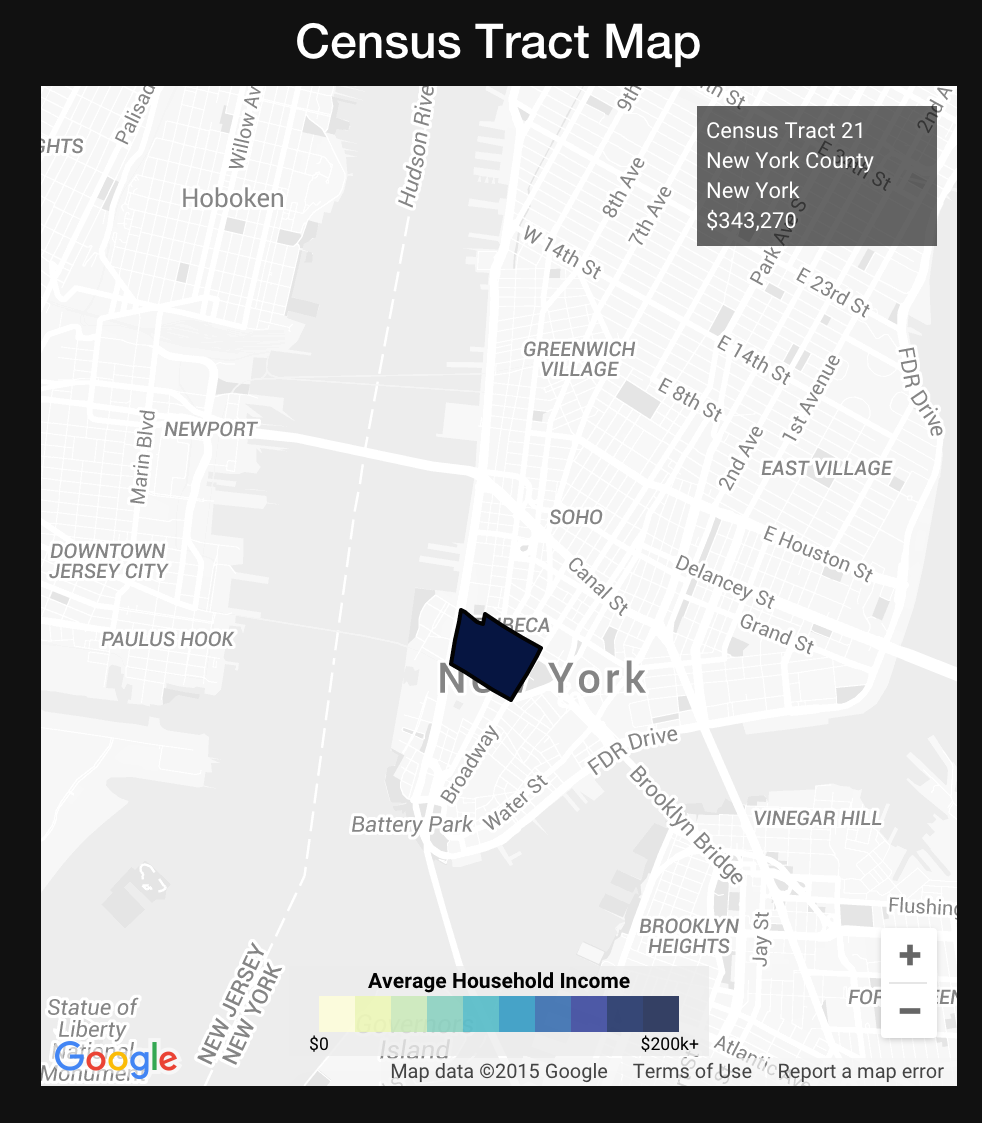
\includegraphics[width=\linewidth]{fig/findyou/tract-map.png}
    \caption{}
  \end{subfigure}
  \caption{(a) Donut graph displaying distribution of income groups visited by user, and (b) map showing tracts visited by user along with income information on each tract.}
\end{figure}


We will begin with a summary of a typical use of FindYou, and proceed to explain each component in more detail, along with the decision-making that influenced the design. 

\textbf{Site Summary} \\
When opening the site, the user is greeted with a general description of the project. After clicking through this screen, the user has the option to import their data from three different web services or to manually import data by clicking visited locations on a map. Upon importing their data, users see the distribution of their visited locations of several different demographic traits, including race, income, age group, and parental status. Finally, at the bottom of the page, users have the ability to donate their data for further research.

\textbf{Design Decisions} \\
\emph{Why did we choose these sites?}
FindYou is currently able to import data from three popular online services or manually, by a user clicking on visited points on a map. The three sites we chose are Instagram, Twitter, and Foursquare. These sites were chosen because they are all popular but also present a diversity of behaviors and different levels of focus on location. We will discuss each of these sites in turn.

\textbf{Foursquare} is a location-based social network and review site. 
Users write reviews of and give tips about locations they have visited. 
It is estimated to have 50 million users. 
Foursquare is the most ``location-centric" of our utilized web-services, as users must reveal their location to obtain any value from the service.
% (TODO: understand what is Swarm and what is Foursquare). 

\textbf{Instagram} is a photo-sharing application owned by Facebook with 400 million monthly active users. 
Instagram is notable for it being primarily targeted at mobile phones; currently users cannot upload photos from a desktop or laptop computer.
The mobile focus makes it is easy for users to ``tag" photos with locations using their phone's GPS device. 
Although many users do tag their photos with location data, unlike Foursquare, it is not necessary to post a location in order to use the app.
Due to the fact that many users do tag their photos with locations, it is the second-most ``location-centric" of our three services.

\textbf{Twitter} is a microblogging service where users post 140 character texts called ``tweets". Twitter has approximately 320 million users. Through its smartphone interface, Twitter users can tag tweets with locations. Many users connect their Twitter account to other web services, such as Foursquare and Instagram, among others, which may also contain location data. The primary focus of most tweets is not about where a user currently is. Therefore, Twitter is the least location-centric. 

We additionally included an option for \textbf{manual input}. 
This option simply has users click on a map to say where they've been. 
We included this option and used this design for several reasons. 
First, we wanted users who do not use any of the three aforementioned services to be able to participate in a location information privacy audit. 
Additionally, allowing users to manually input data gives the ability for users to play with hypothetical trips or to input locations that were not tagged in the services. 
We used this design because it is easy and simple.

In the future, we hope to connect more services and also include more advanced location-data uploading. For example, users could include data in standard geographic formats, such as GeoJSON or those used by GIS software. For the time being, we believe that our three chosen services and simple uploading methodology will provide users with an interesting and useful coverage of options.

\emph{Why did we choose to display these demographic features?}
After a user has imported at least some of their location data, we display demographic information on the places they visited. 
The features we chose to show are race, income level, age, and family make-up (number of households with children). 
The user sees a pie chart showing the average (over the user's visited locations) categorical distribution for that demographic trait. 
The site additionally displays specific details about each category for the user's most visited location. 
Technically, this works by utilizing information from the United States Census. On our server, we store information on the boundaries of each U.S. Census tract. 
We additionally have information on the make-up of each Census tract for our selected traits.
We chose these features to be interesting, surprising, and possible to infer using location data. 
Hopefully, FindYou can include additional interesting demographic features in the future. 

\emph{Why did we use only simple machine learning techniques?}
In addition to descriptive data about the distribution of visits in each category, we also present predictions of which category a user falls into for each demographic attribute. Although users may be interested about the demographics of the locations they visit, they might not realize that this information can be used to infer their own traits. Therefore, showing predictions is useful in and of itself, even if the predictions aren't all accurate, as it shows users that their data can be used in such inferences.
% (TODO: citation to show that users don't understand that most companies use their data?)
Driven by our goal of simplicity in explaining what's going on to the user, we use simple techniques that are intuitive for most users, as opposed to using more difficult to understand methods like SVMs or neural networks. For each demographic trait, we predict the user to be in the class to which they have the most visits. To make this concrete, consider the example of age. We break age into several categories. 
% (TODO: the categories)
We average the distribution of age categories of all the locations a user has visited, and pick the category with the largest proportion. 

\emph{How did you choose to represent locations?}
There are many different ways to represent locations, such as latitude longitudes, venues, cities, or points of interest.
Throughout the paper and the site, we use a United States Census tract as an ``atomic" location.
The United States Census partitions the country into \emph{census tracts}, which are stable geographic boundaries chosen to contain homogeneous populations.
Census tracts are typically the size of a few city blocks and might contain 4000 or fewer people.
We chose to represent all locations as a census tract for several reasons.
First, we can map any latitude longitude point into a census tract, and thus any venue with an associated lat-lon into a tract as well.
Census tracts are small enough to be targeted, but large enough to display without overwhelming the user.
Finally, they are all associated with detailed demographic information from the Census.

Throughout the site, whenever a census tract is mentioned, the user can click on it to see its geographic bounadires and demographic make-up.

\emph{Why only America?}
Due to our reliance on U.S. Census data, our site currently only bases it's predictions on visits to locations in the United States. We hope to expand to other countries in the future. This presents some challenge, as each census of each country will have different types of data available, different classifications, groupings, and currencies, and different APIs. We look forward to tackling this challenge in future work. For the time being, focusing on the world's third most populous country with one standardized census and many online social network users has appeared to be a good option.

